\section{Strategies for categorical data analysis}\label{sec:intro-strat}
Methods of analysis for categorical data can be classified into two
broad categories:
those concerned with hypothesis testing \emph{per se}, and those concerned
with model building.

\subsection{Hypothesis testing approaches}
In many studies, the questions of substantive interest translate readily
into questions concerning hypotheses about association between variables.
If a non-zero association exists, we may wish to characterize the
strength of the association numerically and understand the pattern or
nature of the association.
For example, in \tabref{tab:berk220}, the question
``Is there evidence of gender-bias in admission to graduate school?''
may be expressed in terms of an association between gender and
admission status in a $2 \times 2$ \ctab\
of applicants classified by these two variables.
If so, we can assess the strength of the association by a variety of
measures, including the difference in proportions admitted for men
and women or the ratio of the odds of admission for men compared to
women, as described in \secref{sec:twoway-twobytwo}.

Similarly, in \tabref{tab:arthrit0}, questions about the efficacy of the
treatment for rheumatoid arthritis can be answered in terms of
hypotheses about the associations among the table variables
Treatment, Sex, and the Improvement categories.
Although the main concern might be focused on the overall association between
Treatment and Improvement, one would also wish to know if this association
is the same for men and women.  A stratified analysis (\secref{sec:twoway-strat}) controls for the effects of background
variables like Sex, and tests for \emph{homogeneity of association}
help determine if these associations are equal.

Questions involving tests of such hypotheses are answered most easily
using the randomization-based methods provided by \PROC{FREQ}.
These include the familiar Pearson chi-square,
the Cochran-Mantel-Haenszel test statistics, Fisher's exact test, and a wide variety of measures of strength of association.
These tests make minimal assumptions, principally requiring that subjects
or experimental units have been randomly assigned to the categories of
experimental factors.  The hypothesis testing approach is illustrated
in \chref{ch:twoway}--\ref{ch:corresp}, though the emphasis is on graphical
methods which help to understand the nature of association between
variables.
\begin{Example}[haireye0]{Hair color and eye color}
Two graphical methods related to the hypothesis testing approach
are shown in \figref{fig:haireye0}.
The data concern the relationship between hair color and eye color
in a sample of nearly 600 students (see \tabref{tab:hairdat} and \datref{dat:haireye}).
The standard analysis with \PROC{FREQ} gives a 
Pearson \(\chi^2\) of 138.3 with nine degrees of freedom,
indicating substantial departure from independence.  How do we
understand the {\emph{nature}} of this association between hair
and eye color?

%% two subfig side-by-side
\begin{figure}[htb]
 \begin{minipage}[c]{.49\linewidth}
  \includegraphics[width=1\linewidth,clip]{ch4/fig/mosaic34}
 \end{minipage}%
 \hfill
 \begin{minipage}[c]{.49\linewidth}
  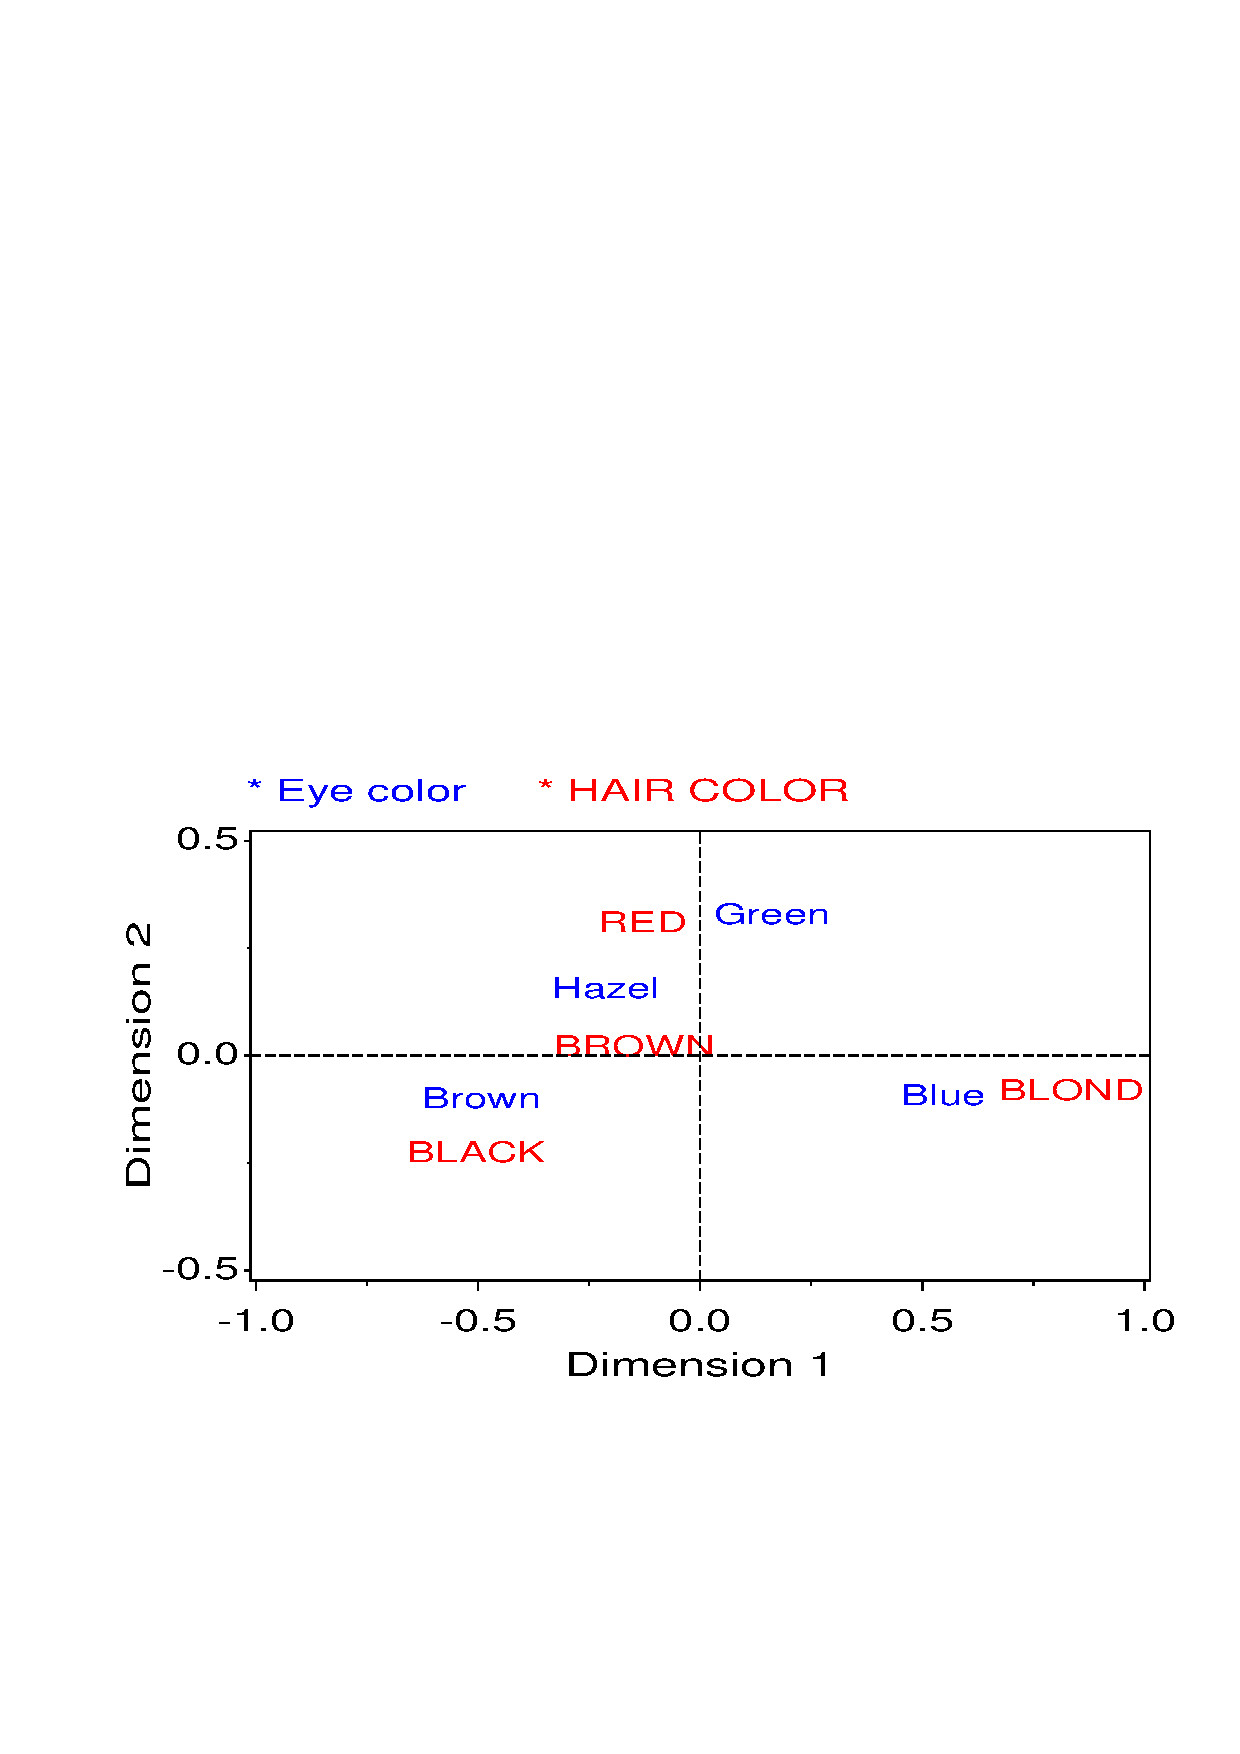
\includegraphics[width=1\linewidth,clip]{ch5/fig/corresp3}
 \end{minipage}
 \caption[Graphical displays for hair color and eye color data]{Graphical displays for hair color and eye color data. Left: mosaic display; right:  correspondence analysis 2D solution.}\label{fig:haireye0}
\end{figure}

The left panel of \figref{fig:haireye0} is a mosaic display
(\chref{ch:mosaic}), constructed so that the size of each rectangle
is proportional to the observed cell frequency. The shading
reflects the cell contribution to the \(\chi^2\) statistic---shades of blue
when the observed frequency is substantially greater than the 
expected frequency under independence, shades of red when the observed freqency
is substantially less, as shown in the legend.

The right panel of this figure shows the results of 
a \CA\ (\chref{ch:corresp}), where the deviations of the hair color and eye
color points from the origin accounts for as much of the \(\chi^2\)
as possible in two dimensions.

We observe that both the hair colors and the eye colors
are ordered from dark to light in the mosaic display and along
Dimension 1 in the \CA\ plot.  The deviations between observed
and expected frequencies have an opposite-corner pattern in the
mosaic display, except for the combination of red hair and green
eyes, which also stand out as the largest values on Dimension 2
in the \CA\ plot.
Displays such as these provide a means to understand \emph{how}
the variables are related.
\end{Example}
 
\subsection{Model building approaches}
In other situations, model-based methods provide tests of equivalent
hypotheses about associations, but (at the cost of additional assumptions)
offer additional advantanges
not provided by the simpler hypotheses-testing approaches.
As in the analysis of quantitative data, linear statistical models
relate the expected value of a response to a linear function of
the table variables, and also assume that residuals or deviations
from the model follow a known parametric form.

For a dichotomous response variable, for example, it is convenient to
construct a model relating a function of the probability, $\pi$,
of one event to a linear combination of the explanatory variables.
Logistic regression uses the logit function,
\begin{equation*}
 \logit ( \pi ) = \log_e \frac { \pi } {1 - \pi}
\end{equation*}
which may be interpreted as the log odds of the given event.

Statistical inferences from model-based methods also provide tests of
hypotheses, but they provide estimates of parameters in the model
and associated confidence intervals and prediction intervals for the 
response as well.  A particular advantage of the logit represention
in the logistic regression model is that estimates of odds ratios
(\secref{sec:twoway-odds})
may be obtained directly from the parameter estimates.

\begin{Example}[nasa0]{Challenger disaster}
\ixd{Challenger disaster|(}
To illustrate, the graph in \figref{fig:nasa1} is based on
a logistic regression model predicting the probability of a
failure in one of the O-ring seals used in the NASA space shuttles
prior to the disasterous launch of the 
\emph{Challenger} in January, 1986.  The explanatory variable is the ambient temperature at the time of the flight.
The sad story behind these data, and the lessons to be learned for
graphical data display are related in \exref{ex:nasa}.
\begin{figure}[htb]
  \centering
  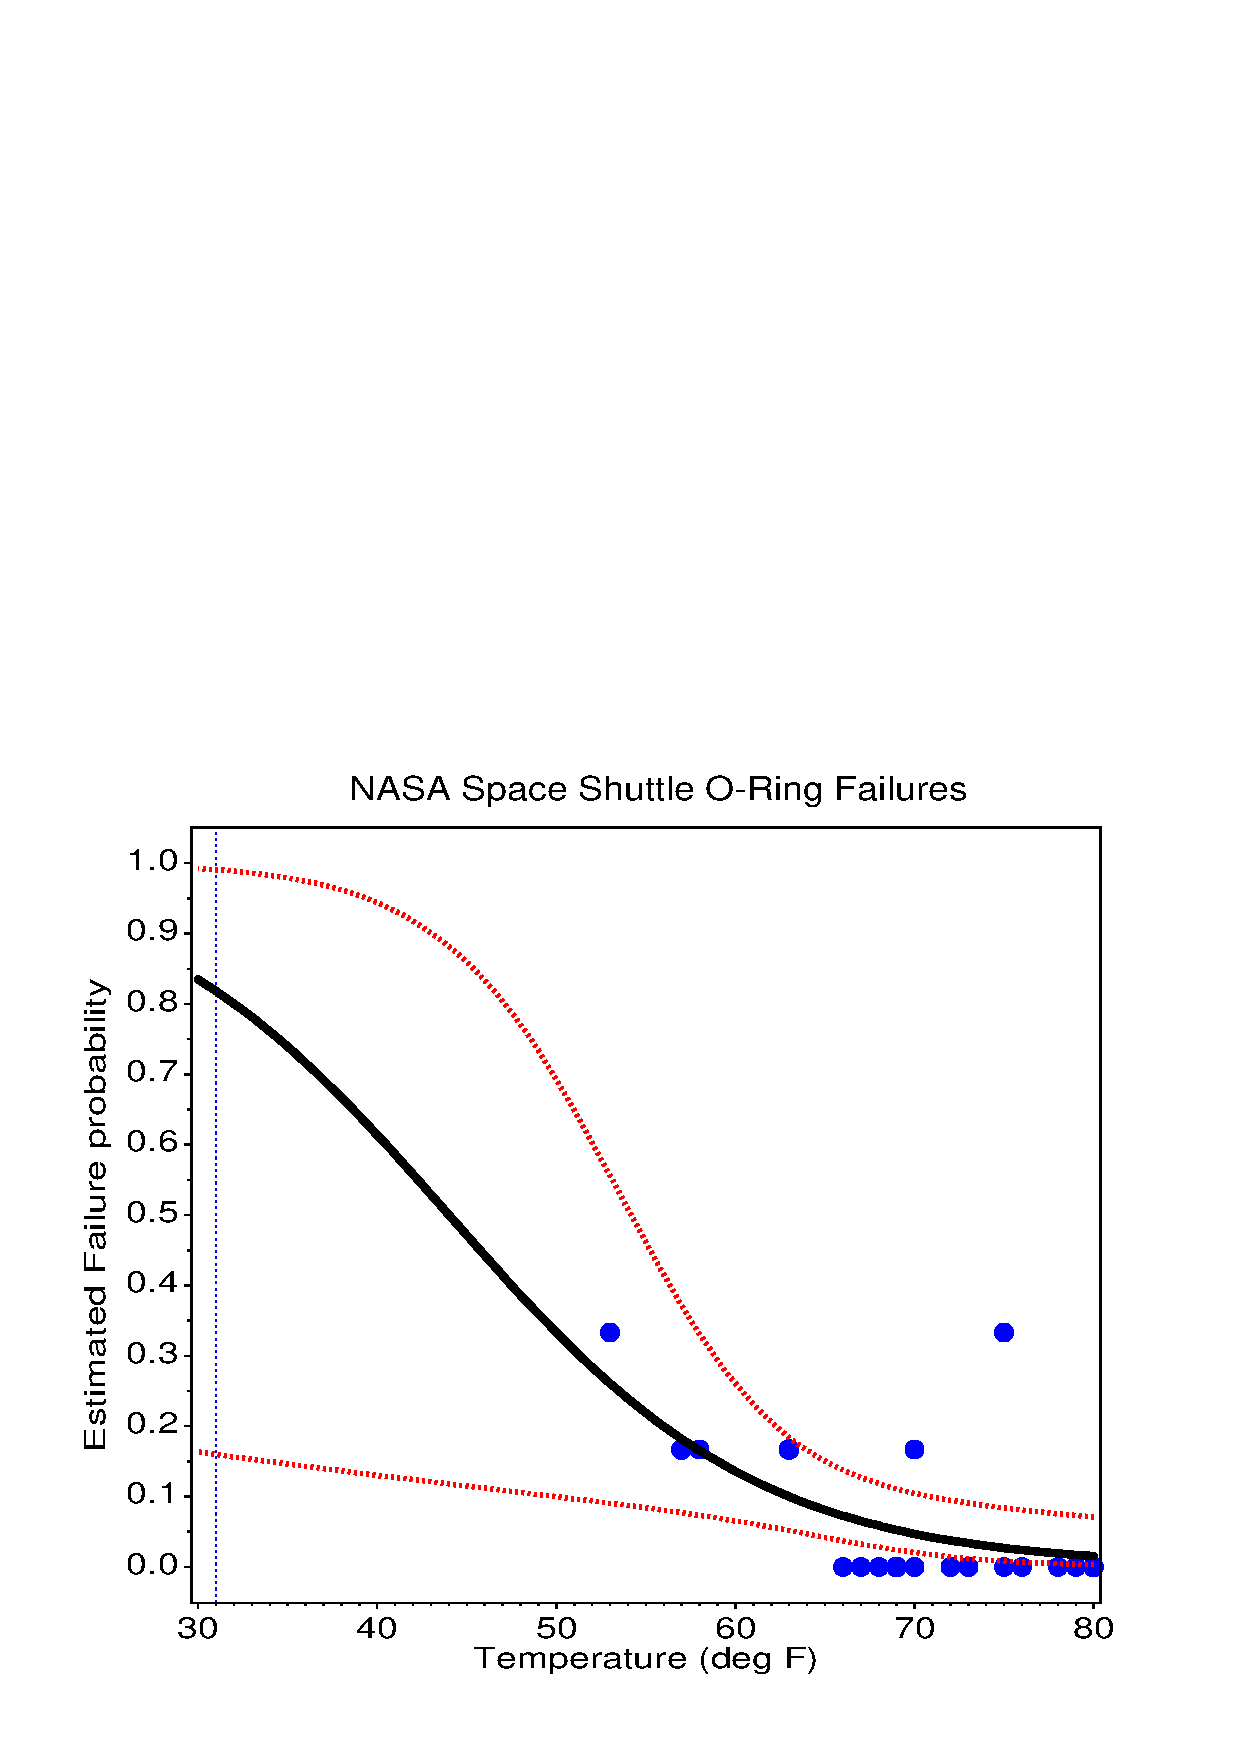
\includegraphics[scale=.6]{ch6/fig/nasa}
  \caption{NASA Space Shuttle 
  O-ring Failure, Observed and Predicted probabilities}\label{fig:nasa1}
\end{figure}

Here, we simply note that the fitted model, shown by the solid line in
\figref{fig:nasa1}, corresponds to the prediction equation
(with standard errors shown in parentheses),
\begin{equation*}
 \logit ( \mbox{Failure} ) =  \cwe{5.09}{3.06} - \cwe{0.116}{0.047} \mbox{ Temp} 
 \end{equation*}%
An hypothesis test that failure probability is unassociated with temperature
is equivalent to the test that the coefficient for temperature in this
model equals 0; this test has a $p$-value of 0.014, convincing evidence
for rejection.
The parameter estimate for temperature, $-0.116$, however, gives more information.  Each \degree{1} increase in temperature decreases the log odds
of failure by 0.116, with 95\% confidence interval ($-0.208$, $-0.0235$).  The equivalent odds ratio is $\exp(-0.116) = 0.891$ (0.812--0.977).
Equivalently, a \degree{10} \emph{decrease} in temperature corresponds to
an odds ratio of a failure of 
$\exp(10 \times 0.116) = 3.18$, more than tripling the odds of a failure.
 
When the \emph{Challenger} was launched, the temperature was only \degree{31}.
The dashed lines in \figref{fig:nasa1} show 95\% prediction intervals
for failure probability.  All previous shuttles (shown by the points
in the figure) had been launched at much warmer temperatures, so the
prediction interval (the dashed vertical line)
at \degree{31} represents a considerable extrapolation
beyond the available data.  Nonetheless, the model building approach
does provide such predictions along with measures of their uncertainty.
\figref{fig:nasa1} is a graph
that might have saved lives.
\ixd{Challenger disaster|)}
\end{Example}

An additional advantage of the model-building approach is that it often
provides greater flexibility and allows more detailed or specialized
descriptions of the relations among variables to be tested.
For instance, in square, two-way tables such as those classifying
the occupations of fathers and sons, or attitudes of husbands and wives,
specialized models dealing with symmetry or forms of lack of symmetry
may be fit and tested.  Such models are usually of much greater
substantive interest than the hypothesis of general association.
Similarly, specialized models for ordinal variables allow more detailed
tests of the nature of association to be examined.
\chref{ch:mosaic} and
\chrange{ch:logistic}{ch:loglin} illustrate many forms of these
specialized models.


%\subsection{Exploratory vs.\ confirmatory analysis}
%A related distinction is that between exploratory and confirmatory
%methods of data analysis.
 

